\section{EXPERIMENTAL RESULTS}
In this section, we show the experimental results to verify the proposed power budgeting method and analyze its energy efficiency and performance. All data are collected on a PC with Intel I5 2400 CPU and 4 GB memory. Multi-core systems with core number ranging from $9$ to $100$ are used in the experiment, and each core with different dark silicon ratio are tested. The thermal models of these multi-core systems are extracted from HotSpot with default package and chip parameters. The ambient temperature are set to be \SI{20}{\degreeCelsius} for all test cases, and the temperature constraint is \SI{95}{\degreeCelsius}.

\subsection{Effectiveness of temperature compensation parameter}
In order to test the effectiveness of the temperature compensation parameter, for example, we first choose a $9$-core system with $4$ active core, the optimal temperature for a specified core with temperature compensation parameter can be computed in \eqref{eq:full_1_ppw} and \eqref{eq:t_ap}. Then, we randomly generate several $4$ active core distributions of a $9$-core system, and compute the real optimal temperature of each of the distribution. Note that the specified core in the previous step is included in the active cores. By comparing the difference of the optimal temperature, the effective of the temperature compensation parameter can be verified.

In addition to the case shown above, we tested many other systems with different number of cores and active cores. The results are collected in Table.x.

\begin{table*}
  \caption{The optimal temperature error induce with and without temperature compensation parameter. The fixed core is the $1^{st}$ core, for each active core number, $50$ random active core distributions are generated.}
  \label{tab:opt_tem}
  \centering
  \begin{tabular}{c|c||p{1cm}<{\centering}|p{1cm}<{\centering}||p{1cm}<{\centering}|p{1cm}<{\centering}}
    \hline
    Core & Active     & \multicolumn{2}{c||}{$T_{err}$($^{\circ}$C)  with $\lambda$}  & \multicolumn{2}{c}{$T_{err}$($^{\circ}$C) without $\lambda$}\\
\cline{3-6}
    \#       &   \#       &  Avg    & Max &  Avg  &  Max  \\
     \hline
\hline
  \multirow{3}{*}{9} &      2       &   1.1  &   1.9 &2.1&4.0\\
             &      4       &    1.3    &   2.7  &7.0&11.7 \\
             &      7       &   1.2     &   2.2   &13.7&16.1\\
     \hline
   \multirow{3}{*}{16} &      3        &   0.3 &   0.7   &1.5 &2.2 \\   
             &      8       &    0.5     &  1.2  &7.2 &8.3   \\
             &      13     &     0.4    &   1.2  &12.9 &13.7 \\
     \hline
  \multirow{3}{*}{25} &      5       &    0.4 & 1.1 & 3.2 &  4.2   \\ 
              &     12      &    0.5     &    1.4   &  8.7 & 9.9 \\
              &     20      &    0.4     &    1.1   & 13.5 & 14.1 \\ 
     \hline
  \multirow{3}{*}{36}  &     8        &    0.4  &    1.1 & 4.1 & 5.6\\
              &     18      &   0.5      &   1.6  & 10.0 & 11.4  \\
              &     28      &    0.4     &   0.9 & 14.4 & 15.2\\
     \hline
  \multirow{3}{*}{64}  &     12      &   0.4  &   1.2  & 3.8 &4.9 \\
              &     32      &    0.5     &     1.6   & 9.6 & 10.6   \\
              &     52      &     0.4   &     1.0   & 15.9 & 16.5\\
 \hline 
\multirow{3}{*}{100}  & 16 & 	 0.5&	1.1& 3.3 &  4.3\\
                      & 52 &	 0.7&	1.7& 11.4 & 13.0\\
                      & 76 &	 0.5&	1.8& 16.6 & 17.6\\
\hline
\end{tabular}
\end{table*}



\begin{figure}
\centering
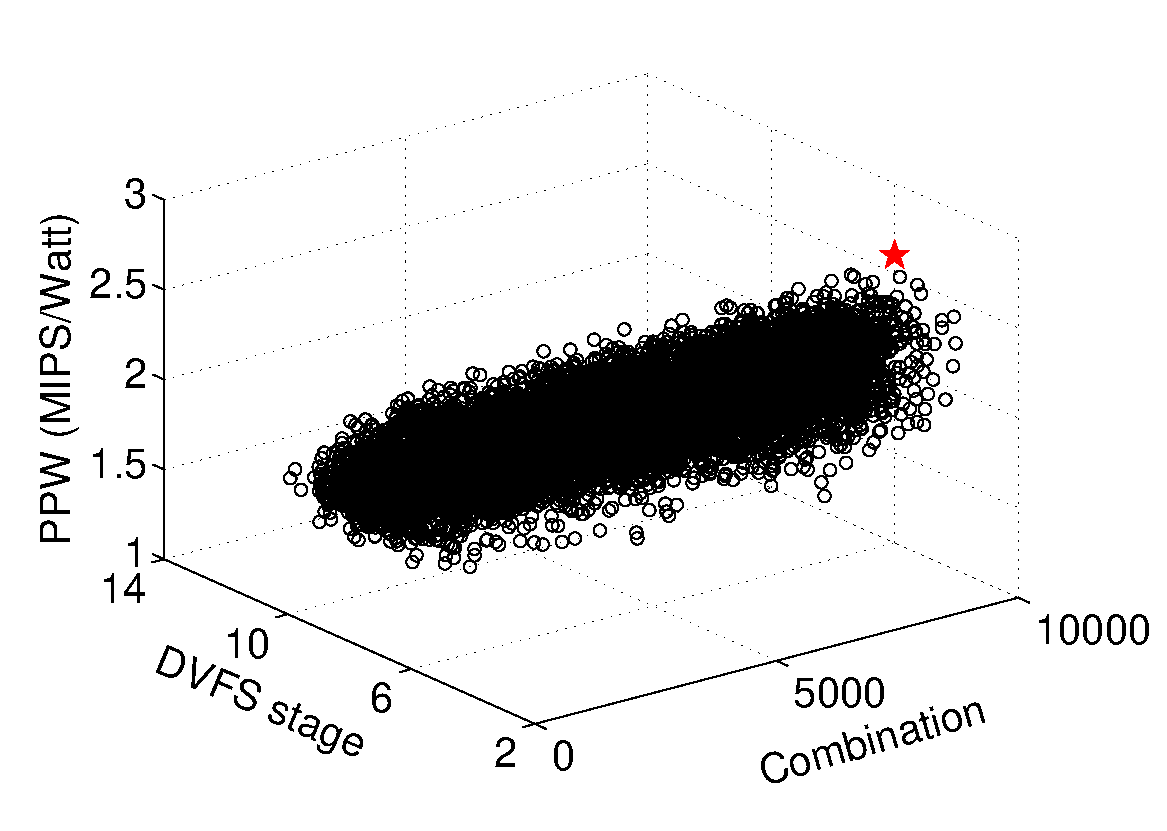
\includegraphics[width=1\linewidth]{fig/best_steady.eps}
\caption{Monte-Carlo of a $16$-core system with $8$ active cores, the variables are the active core distribution and the DVFS stage of each core, the random combination number is 1000, the red pentagram stand for the energy efficiency of our computed power budget}
\end{figure}



\begin{table*}
%  \color{red}
  \caption{Energy efficiency (in MIPS/Watt) and system performance (in MIPS) results comparison of steady state power budgeting. "New" stands for our new power budgeting method, "Monte Carlo" denotes the optimal result with maximum PPW from $1000$ Monte-Carlo simulation with varables being active core distribution and DVFS stage of each active core, and "Random" denotes the averaged result from $10$ random active core distribution with $T_{opt}$ reached for each active core.}
  \label{tab:trans_budget}
  \centering
  \begin{tabular}{c|c||c|c||c|c||c|c}
    \hline
    Core & Active     & \multicolumn{2}{c||}{New} &
                                                    \multicolumn{2}{c||}{Monte-Carlo} & \multicolumn{2}{c} {Random}\\
\cline{3-8}  
\#       &   \#        & PPW & Perf & PPW & Perf  & PPW  & Perf \\
%\#      &   \#         & (W)        &      &   (W)   &    &  (W)    &    &(W)   &  (W)\\
     \hline
\hline
  \multirow{3}{*}{9} &      2     &       2.8    & 137.1     & 3.0    &  91.7    & 2.8 & 118.0\\ 
             &      4             &      2.6     & 227.4    &  2.6  &  183.3    & 2.6 & 186.6\\
             &      7             &       2.4    & 290.2     &  2.3   &  291.7   & 2.4 & 262.3\\
     \hline
\multirow{3}{*}{16}   &      3    &      2.6     & 130.0    &   2.9   &   81.2   &  2.6 & 101.5\\   
             &      8             &      2.6    & 243.3    &   2.5  &    178.1  & 2.5 & 185.2 \\
             &      13            &      2.3     &  270.6   &   2.1  &    318.8  &  2.3 & 237.9\\
     \hline
 \multirow{3}{*}{25}  &      5    &     2.8   &  131.7   &   3.0    &  93.0   & 2.8 &111.8       \\ 
                &     12          &     2.8   &   232.3   &   2.7   &   201.0  & 2.8  & 175.3    \\
                &     20          &     2.7   &   271.2   &   2.5   &  227.3   & 2.7 & 230.5 \\
     \hline
  \multirow{3}{*}{36}  &     8            &      2.8   & 142.0   &  2.9   &  93.8   &  2.8  &111.0    \\
              &     18            &     2.7         & 228.9    &  2.5   &    225.0   &  2.7  & 169.0 \\
              &     28          &        2.6      &   263.2    &  2.4   &    242.2   &  2.6 & 230.2 \\
     \hline
 \multirow{3}{*}{64}   &     12           &     2.7  & 132.2   &   2.8    &  75.0   & 2.7   & 102.7  \\
              &     32      &      2.8      &     230.7     &   2.7    & 196.2   & 2.8   & 210.2  \\
              &     52        &      2.4       & 245.7       &   2.3    &     239.5  & 2.4   & 215.6   \\
              
 \hline 
 \multirow{3}{*}{100} & 16 & 2.8 &  122.6   &   2.7  &  98.2   &   2.8   &   93.1  \\
                      & 52 & 2.7 &  242.1   &   2.5 &  203.5   &   2.7   &   212.5  \\
                      & 76 & 2.4 &  285.7   &  2.3   &  240.6   &   2.4   &   252.8  \\
\hline
  
\end{tabular}
\end{table*}

\subsection{Effectiveness and energy efficiency test for steady state cases}
Due to the high computational complexity of the problem, the optimal active core distribution and the corresponding DVFS stage of each active core for maximum energy efficiency through brute force search is impossible to obtain for multi-core system with large core number. Therefore, in the experiment, we implement the Monte Carlo method. By comparing the energy efficiency of our power budget with the various combinations from Monte Carlo method, we find that the energy efficiency of our computed power budget is close to the optimal one.



\subsection{Energy-efficient power budgeting with optimal performance considering transient effects}

\begin{figure}
\centering
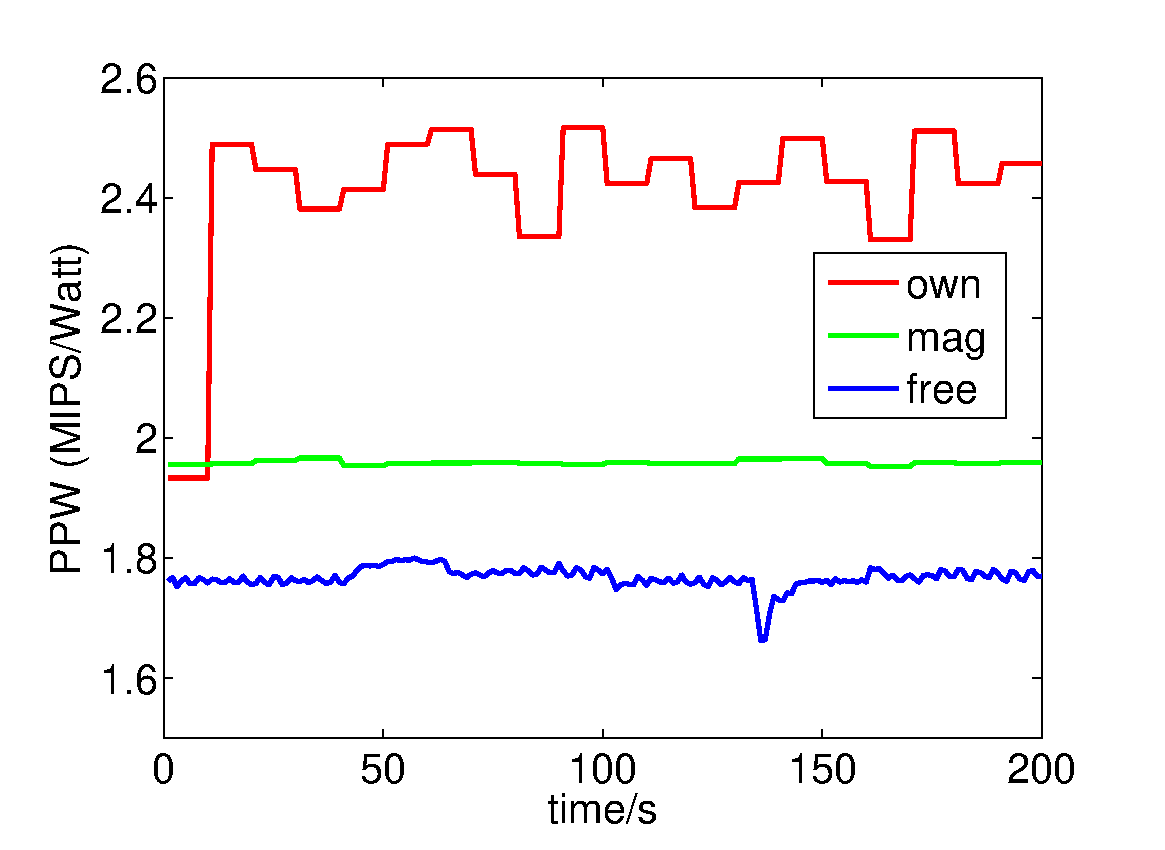
\includegraphics[width=1\linewidth]{fig/PPW.eps}
\caption{PPW}
\end{figure}

\begin{figure}
\centering
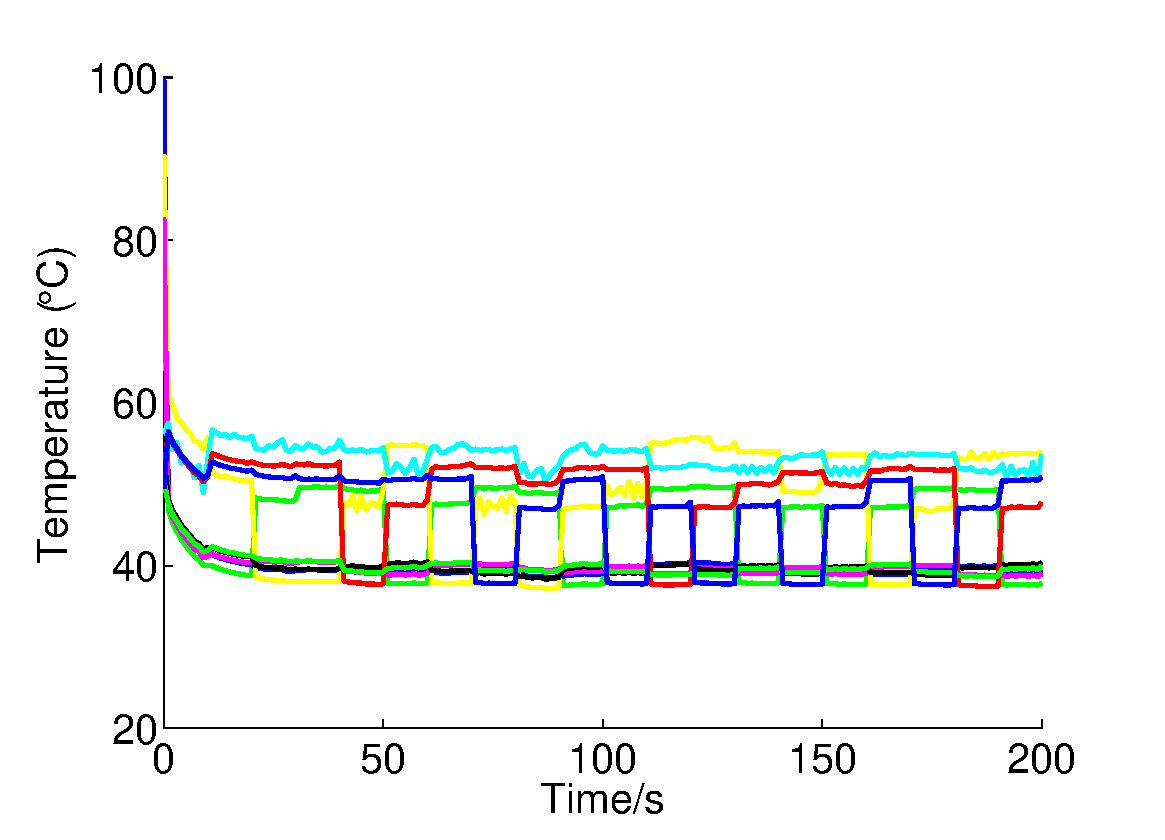
\includegraphics[width=1\linewidth]{fig/tem_own.eps}
\caption{temperature of own}
\end{figure}

\begin{figure}
\centering
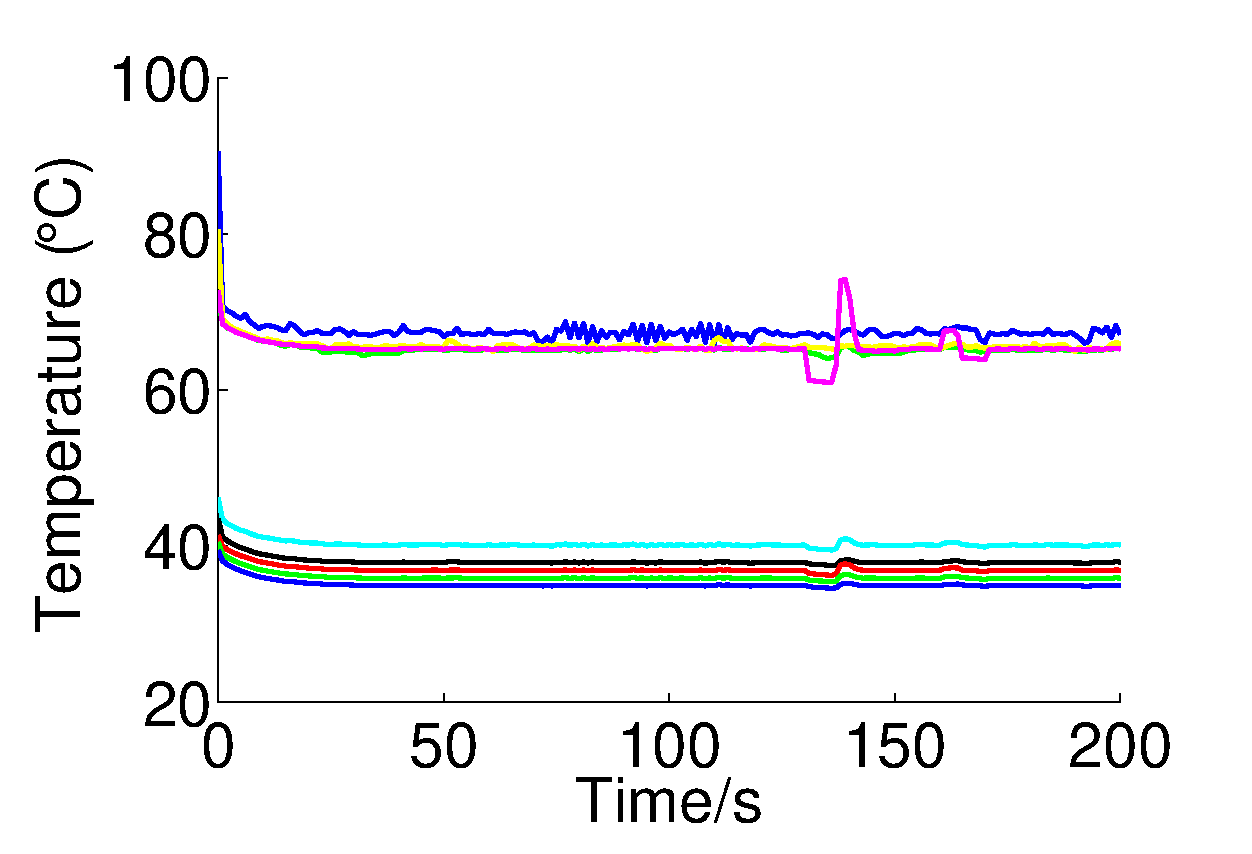
\includegraphics[width=1\linewidth]{fig/tem_mag.eps}
\caption{temperature of mag}
\end{figure}

\begin{figure}
\centering
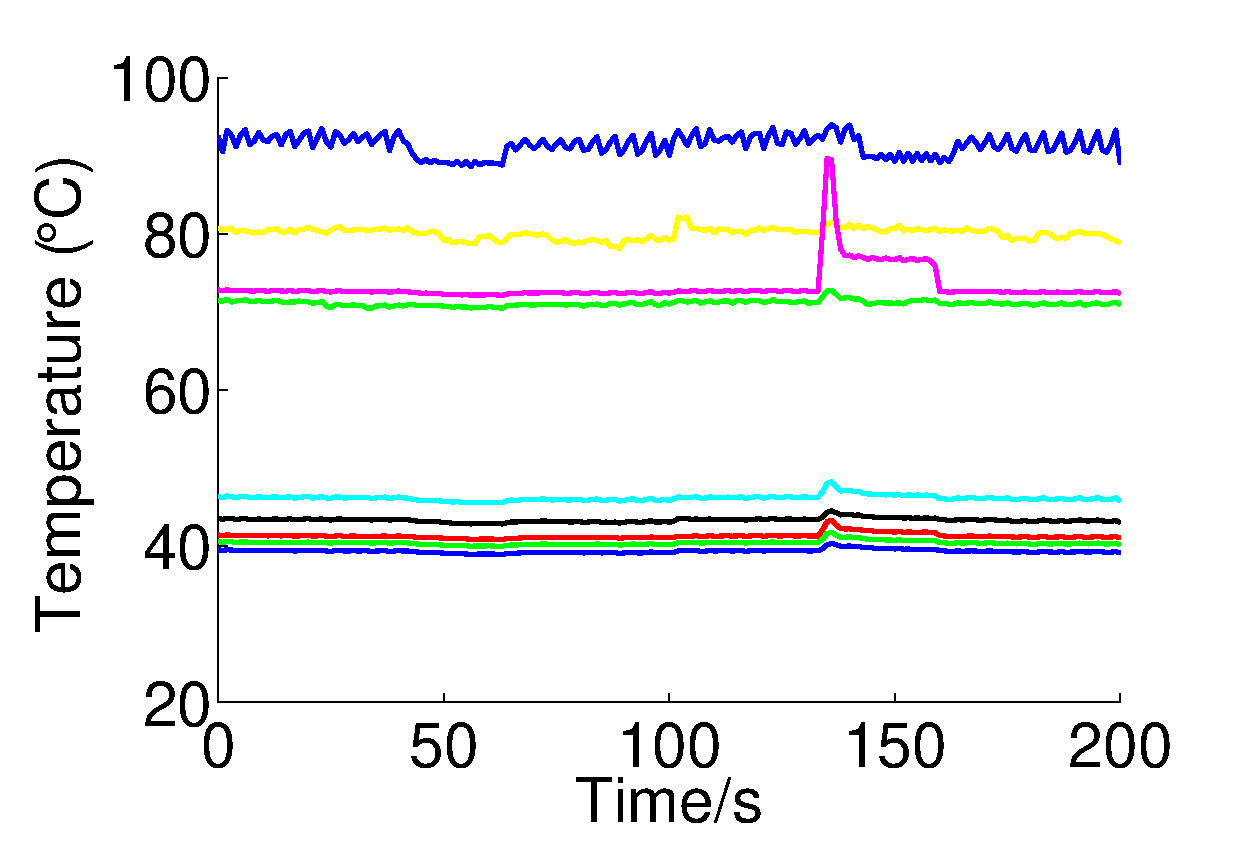
\includegraphics[width=1\linewidth]{fig/tem_free.eps}
\caption{temperature of free}
\end{figure}

Lack one table of dynamic power budgeting's energy efficiency comparison.